\chapter{Experiment}
\label{cha:experiment}
This chapter discusses an experiment, that measures the performance of the previously described authentication mechanisms.
Even if the performance is not the major decision point to choose the correct authentication mechanism, it is still worth considering it.
Especially, because the migration from a monolithic architecture to the microservice architecture already results in a massive performance decrease of around 79.1\%~\cite{ueda2016workload}.
Therefore the performance is already restricted, and the authentication mechanisms should not produce too much overhead.

\section{Setup}
The setup consists of two components, the service, that responds to requests and the client, which performs requests and measures the taken time.
Both components are located in the same network and run on the same machine.
The service is developed in C\# using ASP.Net Core, same as the services of the flea market app, mentioned in chapter~\ref{cha:project_structure}.
The client is a console application, developed in C\# using .NET.
It is not a microservice, but it acts as a service that is located within the deployment.
In a usual deployment it is not good practice to access the services directly from an external application, bypassing the API Gateway.
Nevertheless, for the purpose of an experiment, this is allowed to make the setup simpler and reduce falsifications by other components. 

%The experiment consists of two test cases.
%In the first test case (case A), the console application fetches random numbers from the service.
%Therefore the service does not have to establish any connection to a database.
% TODO: geht das nicht besser ?
%The absolute duration of this test case will not be very meaningful, because it is very unrealistic, that a service considers another service for a task like creating a random number.
%But the trend of this times gives a good value for the comparison of the authentication mechanisms, since the falsification of other operations like accessing a database is minimized.
%In the second case (case B), the console application fetches all users stored in a database table.
%The difference between the two test cases will show how much time has is accounted to the authentication mechanisms and how much time is accounted to other tasks.

The experiment simulates the situation that a service (the console application) performs 1000 requests to another service.
The connection between the console application and the service has to be established, when the first request is performed.
Therefore the first request will take significantly longer, since the full TCP handshake and TLS handshake have to be performed.
Following requests can reuse the already created connection and do not have to perform the whole initialisation process again.
The tests were performed five times to minimize distortions between the test runs.

This experiment does not aim to give and approximation of the expected request durations with the declared technology stack.
Instead it will compare the trends between the authentication mechanisms.
The exact durations are not relevant, since they are influenced by many factors, like the hardware of the components.

Two different implementations of the approach using self-signed JWTs are compared to the performance using mTLS.
First, an implementation of the self-signed JWT approach, in which a new JWT is created for each request is shown.
The second implementation uses the same JWT for all requests.
This should give an idea how the performance using self-signed JWTs can be improved by efficiently reusing the tokens.
Furthermore the experiment includes the response duration without using any authentication mechanism.
This should show how much time is accounted for the authentication mechanisms and how much time is accounted for other tasks like the transport of the request or the generation of the random number.

To simplify the interpretation of the results, the approaches are identified using the identifiers declared in table~\ref{tab:experiment_case_1}.
%\begin{itemize}
%	\item mTLS $\rightarrow \alpha$
%	\item self-signed JWT $\rightarrow \beta$
%	\item self-signed JWT (reusing token) $\rightarrow \gamma$
%	\item none $\rightarrow \delta$
%\end{itemize}
%\begin{table}[H]
%	\centering
%	\begin{tabular}{c|c}
%		\textbf{Authentication Mechanism} & \textbf{Identifier} \\ \hline
%		mTLS & $\alpha$ \\ \hline
%		self-signed JWT & $\beta$ \\ \hline
%		self-signed JWT (reusing token) & $\gamma$ \\ \hline
%		none & $\delta$ \\
%	\end{tabular}
%	\caption{Identifiers for the compared approaches}
%	\label{tab:identifiers}
%\end{table}

\section{Results}

\begin{table}[H]
	\centering
\begin{tabular}{c|c|cc}
	\multicolumn{1}{l|}{\textbf{Authentication Mechanism}} & \textbf{Identifier} & \multicolumn{2}{c}{\textbf{Average Request Duration}} \\ \hline
	\multicolumn{1}{c|}{} & & \multicolumn{1}{c|}{first connection} & reuse connection \\ \hline
	mTLS & $\alpha$ & \multicolumn{1}{c|}{$228.03$ ms} & $9.87$ ms \\ \hline
	self-signed JWT & $\beta$ & \multicolumn{1}{c|}{$193.52$ ms} & $13.57$ ms \\ \hline
	self-signed JWT (reusing token) & $\gamma$ & \multicolumn{1}{c|}{$184.88$ ms} & $8.10$ ms \\ \hline 
	none & $\delta$ & \multicolumn{1}{c|}{$175.78$ ms} & $1.31$ ms
\end{tabular}
\caption{Average request durations of the authentication mechanisms, when random numbers are fetched}
\label{tab:experiment_case_1}
\end{table}

The results of the experiment are shown in table~\ref{tab:experiment_case_1}.
Furthermore the trend of the average request durations is visualized in figure~\ref{fig:trend}.

According to the experiment results $\delta$ is the most efficient approach, because it does not have to handle any additional authentication mechanism.
The first request takes only 175.78 ms in average and the following requests take only 1.31 ms in average.
Comparing $\delta$ with $\alpha$ shows that $\alpha$ takes in average 8.56 ms longer than $\delta$ resulting in a 750\% increase.
Since the authentication is performed only once per request it is not valid to say that the request duration between $\delta$ and $\alpha$ increases by 750\%.
The percentual value is only such significant because the task of generating a random number is very simple.
Therefore only the time offsets of this comparison are interesting.
They show that $\alpha$ increases the request duration by about 8.56 ms on average compared to $\delta$.
The approaches using self-signed JWTs increase the average request duration by 6.79 ms ($\gamma$) to 12.26 ms ($\beta$) on average compared to $\delta$. 

When service-to-service authentication is provided, the lowest duration to establish the first connection is achieved using $\gamma$.
This is reasonable, since $\alpha$ has to perform the extended TLS handshake to transfer the certificate and proove that it owns the corresponding private key.
When self signed-JWTs are used, the services have to proove that they own the private key of the transferred certificate by signing the JWTs.
Therefore the extended handshake is not necessary, for the approaches $\beta$ and $\gamma$.
The results show that $\alpha$ takes about 52.52 ms longer in average than $\gamma$ for establishing the first connection with a service.
$\gamma$ has a minimal advantage of 8.64 ms in average for establishing the first connection compared to $\beta$, because it does not have to create a JWT.

% fake news
%When service-to-service authentication is provided, the lowest duration for the first connection is achieved using mTLS. 
%This is reasonable, since the authentication using self-signed JWTs exchanges the certificate of the client in the first request using the extended TLS handshake same as mTLS.
%Therefore in all three cases the extended TLS handshake has to be performed but the JWT approaches have to attach the JWT additionally.
%The approach that reuses a previously created JWT needs about 10 ms less than the approach in which an new JWT has to be created.
%The first connection using an already created JWT takes still around 16 ms more than the first connection using mTLS.
%This time overhead is caused by the logic that checks the certificate and stores it into the truststore and then checks the validity of the JWT.

Considering the requests after the connection was established, $\gamma$ is the most efficient approach except $\delta$, which does not provide authentication.
Each request takes about 8.10 ms in average which is about 1.23 ms less than using $\alpha$ and 5.47 ms less than $\beta$.
Nevertheless in a more realistic example it is not possbile to reuse the same token for each request.
Therefore using self-signed JWTs would result in a request duration between $\beta$ and $\gamma$ which is around the request duration of $\alpha$.

\begin{figure}
	\centering
	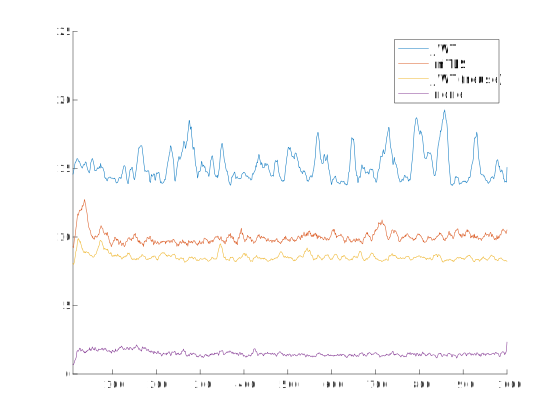
\includegraphics[trim=0 200 0 200, clip, width=\textwidth]{images/experiment/experiment-trend.pdf}
	\caption{Smoothened trend of the average request duration comparing the discussed authentication mechanisms excluding the first request}
	\label{fig:trend}
\end{figure}

\section{Conclusion}
This experiment compared the request durations of the two previously authentication mechanisms.
The results showed that the request durations between the mechanism using self-signed JWTs and mTLS are very similiar.
Depending on the implementation of the JWT approach it can consume up to 34\% more time or up to 20\% less time.
Therefore the performance is not the most crucial criterion when the two authentication mechanisms are compared since it's just a matter of milliseconds. 

Nevertheless for time critical projects in which each millisecond matters, self-signed JWTs are the better choice, since the performance can be optimized in multiple ways.
For example the certificates of the services can be distributed even before the first request is performed.
Or the validity timespan of the tokens can be increased so the same tokens can be used for a longer timespan.
